\begin{question}
\noindent A UI/UX designer is prototyping an icon set on a grid-based canvas. Triangle $J$ has vertices $A(1,1)$, $B(3,1)$ and $C(1,2)$, as shown on the grid below.

\begin{center}
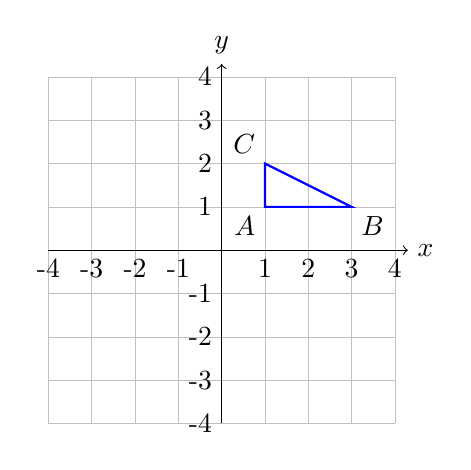
\begin{tikzpicture}[scale=0.55]
    \draw[step=1cm, lightgray, very thin] (-4,-4) grid (4,4);
    \draw[->] (-4,0) -- (4.3,0) node[right]{$x$};
    \draw[->] (0,-4) -- (0,4.3) node[above]{$y$};
    \foreach \x in {-4,-3,-2,-1,1,2,3,4} \node[below] at (\x,0) {\x};
    \foreach \y in {-4,-3,-2,-1,1,2,3,4} \node[left] at (0,\y) {\y};

    \draw[thick, blue] (1,1) -- (3,1) -- (1,2) -- cycle;
    \node[below left] at (1,1) {$A$};
    \node[below right] at (3,1) {$B$};
    \node[above left] at (1,2) {$C$};
\end{tikzpicture}
\end{center}

\begin{enumerate}
    \item[(a)] Triangle $J$ is enlarged by scale factor $-1$, centre $(0,0)$, to give triangle $K$.

    On a copy of the grid, draw and label triangle $K$, and state the coordinates of its vertices $A'$, $B'$ and $C'$.

    \vspace{4cm}
    \answerplain{3}

    \item[(b)] Describe fully the single transformation that maps triangle $J$ directly onto triangle $K$.

    \vspace{3cm}
    \answerlines{2}{2}
\end{enumerate}
\end{question}
